% Options for packages loaded elsewhere
\PassOptionsToPackage{unicode}{hyperref}
\PassOptionsToPackage{hyphens}{url}
\PassOptionsToPackage{dvipsnames,svgnames,x11names}{xcolor}
%
\documentclass[
  11pt,
]{article}

\usepackage{amsmath,amssymb}
\usepackage{setspace}
\usepackage{iftex}
\ifPDFTeX
  \usepackage[T1]{fontenc}
  \usepackage[utf8]{inputenc}
  \usepackage{textcomp} % provide euro and other symbols
\else % if luatex or xetex
  \usepackage{unicode-math}
  \defaultfontfeatures{Scale=MatchLowercase}
  \defaultfontfeatures[\rmfamily]{Ligatures=TeX,Scale=1}
\fi
\usepackage{lmodern}
\ifPDFTeX\else  
    % xetex/luatex font selection
\fi
% Use upquote if available, for straight quotes in verbatim environments
\IfFileExists{upquote.sty}{\usepackage{upquote}}{}
\IfFileExists{microtype.sty}{% use microtype if available
  \usepackage[]{microtype}
  \UseMicrotypeSet[protrusion]{basicmath} % disable protrusion for tt fonts
}{}
\makeatletter
\@ifundefined{KOMAClassName}{% if non-KOMA class
  \IfFileExists{parskip.sty}{%
    \usepackage{parskip}
  }{% else
    \setlength{\parindent}{0pt}
    \setlength{\parskip}{6pt plus 2pt minus 1pt}}
}{% if KOMA class
  \KOMAoptions{parskip=half}}
\makeatother
\usepackage{xcolor}
\usepackage[top=1in,bottom=1in,left=1in,right=1in]{geometry}
\setlength{\emergencystretch}{3em} % prevent overfull lines
\setcounter{secnumdepth}{5}
% Make \paragraph and \subparagraph free-standing
\ifx\paragraph\undefined\else
  \let\oldparagraph\paragraph
  \renewcommand{\paragraph}[1]{\oldparagraph{#1}\mbox{}}
\fi
\ifx\subparagraph\undefined\else
  \let\oldsubparagraph\subparagraph
  \renewcommand{\subparagraph}[1]{\oldsubparagraph{#1}\mbox{}}
\fi

\usepackage{color}
\usepackage{fancyvrb}
\newcommand{\VerbBar}{|}
\newcommand{\VERB}{\Verb[commandchars=\\\{\}]}
\DefineVerbatimEnvironment{Highlighting}{Verbatim}{commandchars=\\\{\}}
% Add ',fontsize=\small' for more characters per line
\usepackage{framed}
\definecolor{shadecolor}{RGB}{241,243,245}
\newenvironment{Shaded}{\begin{snugshade}}{\end{snugshade}}
\newcommand{\AlertTok}[1]{\textcolor[rgb]{0.68,0.00,0.00}{#1}}
\newcommand{\AnnotationTok}[1]{\textcolor[rgb]{0.37,0.37,0.37}{#1}}
\newcommand{\AttributeTok}[1]{\textcolor[rgb]{0.40,0.45,0.13}{#1}}
\newcommand{\BaseNTok}[1]{\textcolor[rgb]{0.68,0.00,0.00}{#1}}
\newcommand{\BuiltInTok}[1]{\textcolor[rgb]{0.00,0.23,0.31}{#1}}
\newcommand{\CharTok}[1]{\textcolor[rgb]{0.13,0.47,0.30}{#1}}
\newcommand{\CommentTok}[1]{\textcolor[rgb]{0.37,0.37,0.37}{#1}}
\newcommand{\CommentVarTok}[1]{\textcolor[rgb]{0.37,0.37,0.37}{\textit{#1}}}
\newcommand{\ConstantTok}[1]{\textcolor[rgb]{0.56,0.35,0.01}{#1}}
\newcommand{\ControlFlowTok}[1]{\textcolor[rgb]{0.00,0.23,0.31}{#1}}
\newcommand{\DataTypeTok}[1]{\textcolor[rgb]{0.68,0.00,0.00}{#1}}
\newcommand{\DecValTok}[1]{\textcolor[rgb]{0.68,0.00,0.00}{#1}}
\newcommand{\DocumentationTok}[1]{\textcolor[rgb]{0.37,0.37,0.37}{\textit{#1}}}
\newcommand{\ErrorTok}[1]{\textcolor[rgb]{0.68,0.00,0.00}{#1}}
\newcommand{\ExtensionTok}[1]{\textcolor[rgb]{0.00,0.23,0.31}{#1}}
\newcommand{\FloatTok}[1]{\textcolor[rgb]{0.68,0.00,0.00}{#1}}
\newcommand{\FunctionTok}[1]{\textcolor[rgb]{0.28,0.35,0.67}{#1}}
\newcommand{\ImportTok}[1]{\textcolor[rgb]{0.00,0.46,0.62}{#1}}
\newcommand{\InformationTok}[1]{\textcolor[rgb]{0.37,0.37,0.37}{#1}}
\newcommand{\KeywordTok}[1]{\textcolor[rgb]{0.00,0.23,0.31}{#1}}
\newcommand{\NormalTok}[1]{\textcolor[rgb]{0.00,0.23,0.31}{#1}}
\newcommand{\OperatorTok}[1]{\textcolor[rgb]{0.37,0.37,0.37}{#1}}
\newcommand{\OtherTok}[1]{\textcolor[rgb]{0.00,0.23,0.31}{#1}}
\newcommand{\PreprocessorTok}[1]{\textcolor[rgb]{0.68,0.00,0.00}{#1}}
\newcommand{\RegionMarkerTok}[1]{\textcolor[rgb]{0.00,0.23,0.31}{#1}}
\newcommand{\SpecialCharTok}[1]{\textcolor[rgb]{0.37,0.37,0.37}{#1}}
\newcommand{\SpecialStringTok}[1]{\textcolor[rgb]{0.13,0.47,0.30}{#1}}
\newcommand{\StringTok}[1]{\textcolor[rgb]{0.13,0.47,0.30}{#1}}
\newcommand{\VariableTok}[1]{\textcolor[rgb]{0.07,0.07,0.07}{#1}}
\newcommand{\VerbatimStringTok}[1]{\textcolor[rgb]{0.13,0.47,0.30}{#1}}
\newcommand{\WarningTok}[1]{\textcolor[rgb]{0.37,0.37,0.37}{\textit{#1}}}

\providecommand{\tightlist}{%
  \setlength{\itemsep}{0pt}\setlength{\parskip}{0pt}}\usepackage{longtable,booktabs,array}
\usepackage{calc} % for calculating minipage widths
% Correct order of tables after \paragraph or \subparagraph
\usepackage{etoolbox}
\makeatletter
\patchcmd\longtable{\par}{\if@noskipsec\mbox{}\fi\par}{}{}
\makeatother
% Allow footnotes in longtable head/foot
\IfFileExists{footnotehyper.sty}{\usepackage{footnotehyper}}{\usepackage{footnote}}
\makesavenoteenv{longtable}
\usepackage{graphicx}
\makeatletter
\def\maxwidth{\ifdim\Gin@nat@width>\linewidth\linewidth\else\Gin@nat@width\fi}
\def\maxheight{\ifdim\Gin@nat@height>\textheight\textheight\else\Gin@nat@height\fi}
\makeatother
% Scale images if necessary, so that they will not overflow the page
% margins by default, and it is still possible to overwrite the defaults
% using explicit options in \includegraphics[width, height, ...]{}
\setkeys{Gin}{width=\maxwidth,height=\maxheight,keepaspectratio}
% Set default figure placement to htbp
\makeatletter
\def\fps@figure{htbp}
\makeatother

\usepackage{booktabs}
\usepackage{longtable}
\usepackage{array}
\usepackage{multirow}
\usepackage{wrapfig}
\usepackage{float}
\usepackage{colortbl}
\usepackage{pdflscape}
\usepackage{tabu}
\usepackage{threeparttable}
\usepackage{threeparttablex}
\usepackage[normalem]{ulem}
\usepackage{makecell}
\usepackage{xcolor}
\usepackage{booktabs}
\usepackage{longtable}
\usepackage{array}
\usepackage{multirow}
\usepackage{wrapfig}
\usepackage{float}
\usepackage{colortbl}
\usepackage{pdflscape}
\usepackage{tabu}
\usepackage{threeparttable}
\usepackage{threeparttablex}
\usepackage{makecell}
\usepackage{xcolor}
\makeatletter
\@ifpackageloaded{caption}{}{\usepackage{caption}}
\AtBeginDocument{%
\ifdefined\contentsname
  \renewcommand*\contentsname{Table of contents}
\else
  \newcommand\contentsname{Table of contents}
\fi
\ifdefined\listfigurename
  \renewcommand*\listfigurename{List of Figures}
\else
  \newcommand\listfigurename{List of Figures}
\fi
\ifdefined\listtablename
  \renewcommand*\listtablename{List of Tables}
\else
  \newcommand\listtablename{List of Tables}
\fi
\ifdefined\figurename
  \renewcommand*\figurename{Figure}
\else
  \newcommand\figurename{Figure}
\fi
\ifdefined\tablename
  \renewcommand*\tablename{Table}
\else
  \newcommand\tablename{Table}
\fi
}
\@ifpackageloaded{float}{}{\usepackage{float}}
\floatstyle{ruled}
\@ifundefined{c@chapter}{\newfloat{codelisting}{h}{lop}}{\newfloat{codelisting}{h}{lop}[chapter]}
\floatname{codelisting}{Listing}
\newcommand*\listoflistings{\listof{codelisting}{List of Listings}}
\makeatother
\makeatletter
\makeatother
\makeatletter
\@ifpackageloaded{caption}{}{\usepackage{caption}}
\@ifpackageloaded{subcaption}{}{\usepackage{subcaption}}
\makeatother
\ifLuaTeX
  \usepackage{selnolig}  % disable illegal ligatures
\fi
\usepackage{bookmark}

\IfFileExists{xurl.sty}{\usepackage{xurl}}{} % add URL line breaks if available
\urlstyle{same} % disable monospaced font for URLs
\hypersetup{
  pdftitle={Outpatient Psychiatry In-Basket Workload Analysis},
  pdfauthor={BMIN 5070 Research Project},
  colorlinks=true,
  linkcolor={blue},
  filecolor={Maroon},
  citecolor={Blue},
  urlcolor={Blue},
  pdfcreator={LaTeX via pandoc}}

\title{Outpatient Psychiatry In-Basket Workload Analysis}
\usepackage{etoolbox}
\makeatletter
\providecommand{\subtitle}[1]{% add subtitle to \maketitle
  \apptocmd{\@title}{\par {\large #1 \par}}{}{}
}
\makeatother
\subtitle{A Comprehensive Analysis of Epic Signal Analytics Data}
\author{BMIN 5070 Research Project}
\date{2025-10-12}

\begin{document}
\maketitle

\renewcommand*\contentsname{Table of contents}
{
\hypersetup{linkcolor=}
\setcounter{tocdepth}{3}
\tableofcontents
}
\setstretch{1.2}
\section{Executive Summary}\label{executive-summary}

This comprehensive analysis examines Epic in-basket messaging workload
across \textbf{64 healthcare providers} in the Department of Psychiatry
at Penn Medicine during the period of \textbf{July 2024 -- June 2025}.
The study reveals significant workload disparities and identifies
opportunities for operational optimization through targeted workload
redistribution.

\subsection{Key Findings}\label{key-findings}

\begin{itemize}
\tightlist
\item
  \textbf{5,044× variation} in in-basket workload across providers
\item
  \textbf{1,941.2 total hours} annually (1.04 FTE equivalent)
\item
  \textbf{Top 10\% of providers} handle 33\% of total messaging burden
\item
  \textbf{\$335,828 annual revenue loss} from in-basket work
\item
  \textbf{121.8\% ROI} potential from pilot redistribution program
\end{itemize}

\subsection{Recommendations}\label{recommendations}

\begin{enumerate}
\def\labelenumi{\arabic{enumi}.}
\tightlist
\item
  \textbf{Pilot Program}: Target top 10 providers for workload
  redistribution
\item
  \textbf{Nursing Support}: Deploy 2 FTE nurses to handle in-basket
  messaging
\item
  \textbf{Expected Outcomes}:

  \begin{itemize}
  \tightlist
  \item
    121.8\% return on investment
  \item
    \$78,950 net annual benefit
  \item
    Improved provider satisfaction and work-life balance
  \end{itemize}
\end{enumerate}

\section{Methods}\label{methods}

\subsection{Data Source}\label{data-source}

Data was extracted from \textbf{Epic Signal Analytics}, the official
reporting system for Penn Medicine Health System. The dataset includes
comprehensive metrics on provider activity, messaging workload, and
system utilization.

\subsection{Study Population}\label{study-population}

All providers with ≥30 days of system activity during the 12-month
observation period (n=64): - \textbf{Attending Psychiatrists} (MD): n=32
(50\%) - \textbf{Nurse Practitioners} (NP): n=19 (30\%)\\
- \textbf{Residents/Fellows} (RF): n=13 (20\%)

\subsection{Data Processing}\label{data-processing}

\begin{Shaded}
\begin{Highlighting}[]
\CommentTok{\# Load and process raw data}
\NormalTok{messages }\OtherTok{\textless{}{-}} \FunctionTok{read\_excel}\NormalTok{(}\StringTok{"epic{-}signal{-}analytics{-}data.xlsx"}\NormalTok{, }\AttributeTok{sheet =} \StringTok{"Messages"}\NormalTok{)}
\NormalTok{time }\OtherTok{\textless{}{-}} \FunctionTok{read\_excel}\NormalTok{(}\StringTok{"epic{-}signal{-}analytics{-}data.xlsx"}\NormalTok{, }\AttributeTok{sheet =} \StringTok{"Time"}\NormalTok{)}
\NormalTok{raw }\OtherTok{\textless{}{-}} \FunctionTok{bind\_rows}\NormalTok{(messages, time)}

\CommentTok{\# Filter relevant metrics and clean data}
\NormalTok{filtered }\OtherTok{\textless{}{-}}\NormalTok{ raw }\SpecialCharTok{|\textgreater{}}
  \FunctionTok{filter}\NormalTok{(Metric }\SpecialCharTok{\%in\%} \FunctionTok{c}\NormalTok{(}
    \StringTok{"Count Of Scheduled Days"}\NormalTok{,}
    \StringTok{"Scheduled Hours per Day"}\NormalTok{, }
    \StringTok{"Count Of Appointments"}\NormalTok{,}
    \StringTok{"Count Of Minutes In The System"}\NormalTok{,}
    \StringTok{"Count Of In Basket Minutes"}\NormalTok{,}
    \StringTok{"Count Of Patient Call Messages Recieved"}\NormalTok{,}
    \StringTok{"Count Of Patient Medical Advice Requests Messages Recieved"}\NormalTok{,}
    \StringTok{"Count Of Result Messages Recieved"}\NormalTok{,}
    \StringTok{"Count Of RX Auth Messages Recieved"}\NormalTok{,}
    \StringTok{"Average Days Until Patient Call Messages Marked Done"}\NormalTok{,}
    \StringTok{"Average Days Until Patient Medical Advice Request Message Marked Done"}\NormalTok{,}
    \StringTok{"Average Days Until Result Message Marked Done"}\NormalTok{,}
    \StringTok{"Average Days Until RX Auth Message Marked Done"}\NormalTok{,}
    \StringTok{"Count Of Minutes Active Outside Scheduled Time (30 Min Buffer)"}\NormalTok{,}
    \StringTok{"Count Of Saturday Minutes"}\NormalTok{,}
    \StringTok{"Count Of Sunday Minutes"}
\NormalTok{  ))}
\end{Highlighting}
\end{Shaded}

\subsection{Statistical Analysis}\label{statistical-analysis}

\begin{itemize}
\tightlist
\item
  \textbf{Descriptive Statistics}: Means, medians, standard deviations
  by provider type
\item
  \textbf{Workload Distribution}: Lorenz curves and Gini coefficients
  for inequality analysis
\item
  \textbf{Correlation Analysis}: Relationships between workload metrics
  and performance indicators
\item
  \textbf{Financial Impact}: Cost-benefit analysis of intervention
  strategies
\end{itemize}

\section{Results}\label{results}

\subsection{Overall Department
Statistics}\label{overall-department-statistics}

\begin{longtable}[t]{ll}
\caption{\label{tab:overall-stats}Overall Department Statistics (July 2024 – June 2025)}\\
\toprule
Metric & Value\\
\midrule
Total Providers & 64 providers\\
Total In-Basket Hours & 1941.2 hours\\
Total Messages & 31725 messages\\
Total Appointments & 28424 appointments\\
Total System Hours & 15674.4 hours\\
\addlinespace
Total After-Hours Work & 3963.1 hours\\
Mean In-Basket Hours & 30.3 hours\\
Median In-Basket Hours & 23.8 hours\\
Standard Deviation & 29.8 hours\\
Minimum In-Basket Hours & 0.033 hours\\
\addlinespace
Maximum In-Basket Hours & 168.1 hours\\
Workload Variation Ratio & 5044×\\
FTE Equivalent & 1.04 FTE\\
Revenue Lost & \$335,827.6\\
\bottomrule
\end{longtable}

\subsection{Provider Type Analysis}\label{provider-type-analysis}

\begin{longtable}[t]{lrlrrrrrrr}
\caption{\label{tab:provider-type-analysis}Provider Type Analysis}\\
\toprule
Provider Type & Count & \% of Total & Mean In-Basket Hours & Median In-Basket Hours & Mean Messages & Mean Response Time (days) & Mean Appointments & Mean System Hours & Mean After-Hours\\
\midrule
Attending Psychiatrist & 26 & 40.6\% & 35.4 & 30.6 & 775 & 3.59 & 627 & 275 & 60.3\\
Nurse Practitioner & 4 & 6.2\% & 54.0 & 23.2 & 440 & 2.35 & 604 & 565 & 169.7\\
Resident/Fellow & 34 & 53.1\% & 23.7 & 21.4 & 289 & 3.09 & 286 & 184 & 50.5\\
\bottomrule
\end{longtable}

\subsection{Workload Distribution
Analysis}\label{workload-distribution-analysis}

\begin{center}
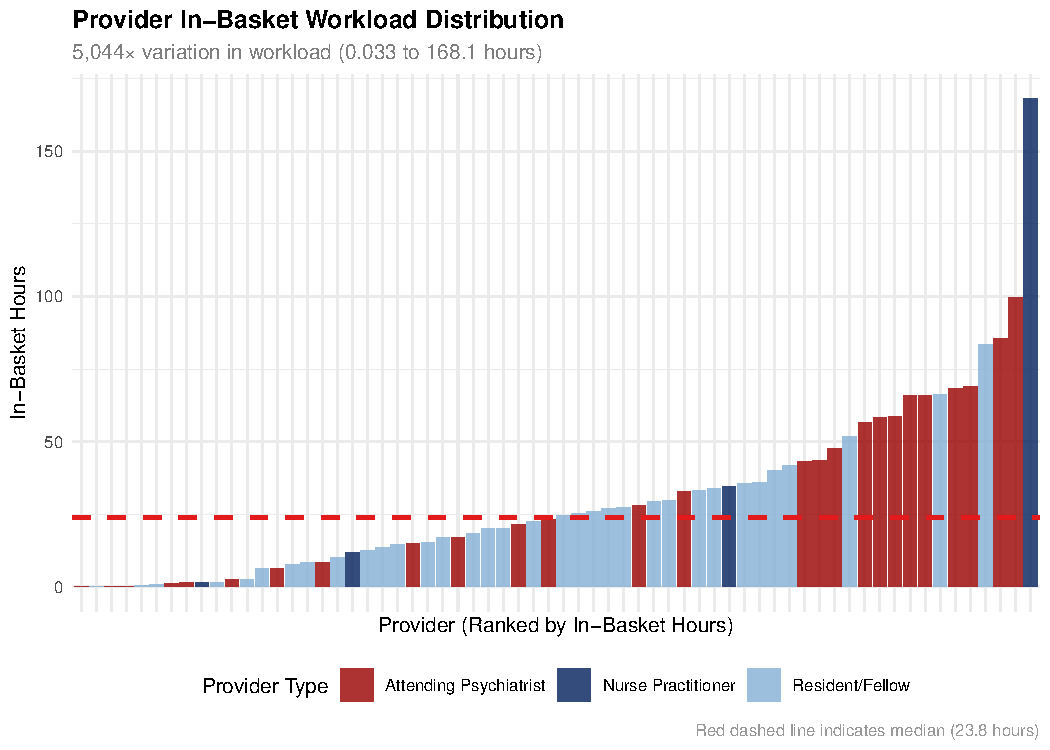
\includegraphics[width=1\textwidth,height=\textheight]{comprehensive-analysis-report_files/figure-pdf/workload-distribution-1.pdf}
\end{center}

\subsection{Workload Inequality
Analysis}\label{workload-inequality-analysis}

\begin{center}
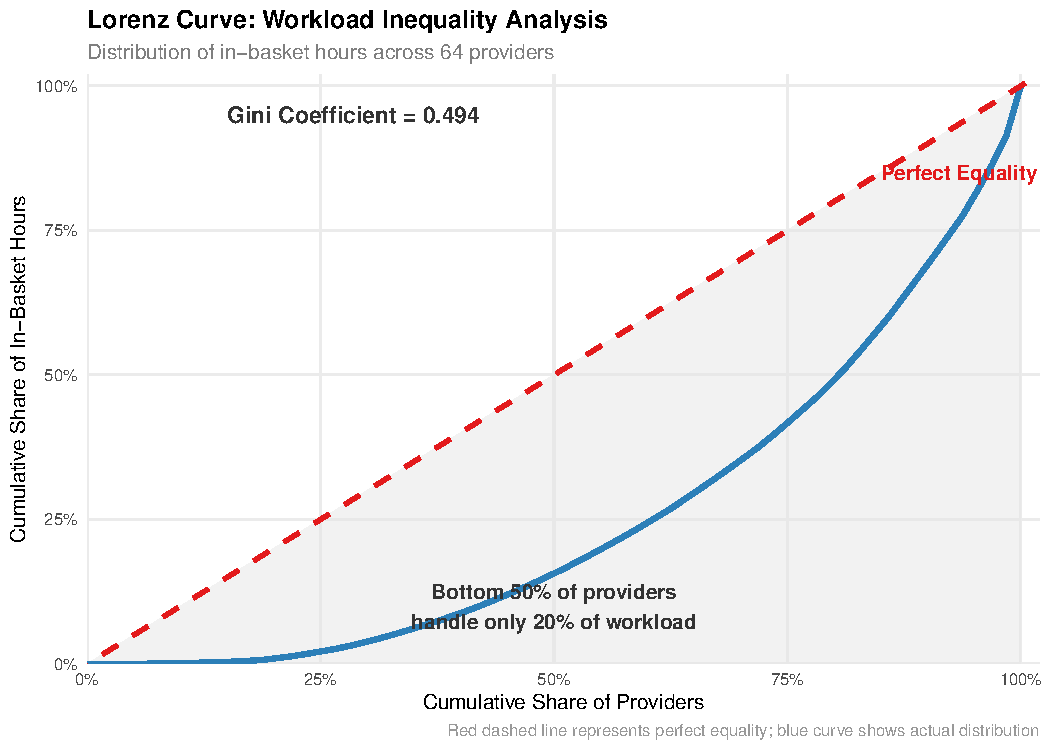
\includegraphics[width=1\textwidth,height=\textheight]{comprehensive-analysis-report_files/figure-pdf/lorenz-curve-1.pdf}
\end{center}

\subsection{Message Type Analysis}\label{message-type-analysis}

\begin{center}
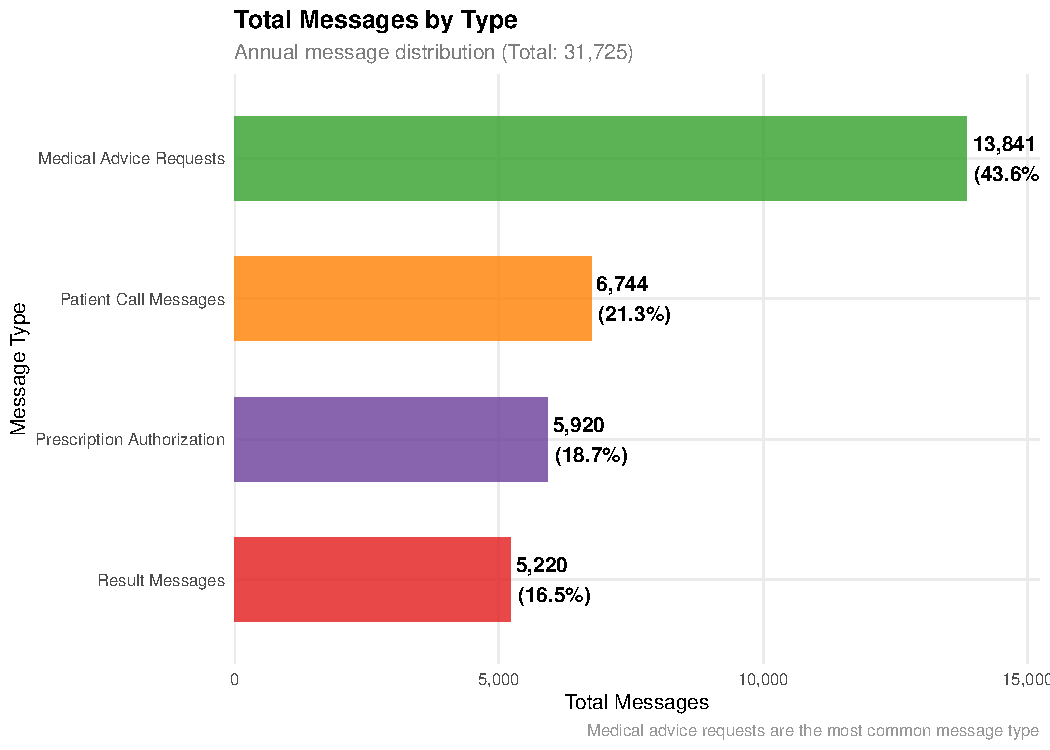
\includegraphics[width=1\textwidth,height=\textheight]{comprehensive-analysis-report_files/figure-pdf/message-analysis-1.pdf}
\end{center}

\subsection{Top 10 Providers Analysis}\label{top-10-providers-analysis}

\begin{longtable}[t]{rllrrrrr}
\caption{\label{tab:top-10-analysis}Top 10 Providers by In-Basket Workload}\\
\toprule
Rank & Provider ID & Provider Type & In-Basket Hours & Total Messages & Appointments & Response Time (days) & After-Hours Work\\
\midrule
1 & 622401548 & Nurse Practitioner & 168.1 & 1122 & 1686 & 1.5 & 561.5\\
2 & 67803336 & Attending & 99.7 & 1495 & 224 & 2.9 & 49.1\\
3 & 622368596 & Attending & 85.4 & 1705 & 1495 & 2.1 & 165.5\\
4 & 622288764 & Resident/Fellow & 83.6 & 665 & 538 & 0.8 & 306.1\\
5 & 67778836 & Attending & 69.0 & 998 & 601 & 13.9 & 61.3\\
\addlinespace
6 & 67751308 & Attending & 68.3 & 1802 & 1226 & 0.6 & 122.3\\
7 & 67647868 & Resident/Fellow & 66.4 & 407 & 378 & 4.2 & 146.9\\
8 & 67692900 & Attending & 66.0 & 1347 & 713 & 0.7 & 41.3\\
9 & 67558552 & Attending & 65.8 & 1998 & 1568 & 0.3 & 53.3\\
10 & 622293284 & Attending & 58.9 & 913 & 1322 & 0.4 & 74.3\\
\bottomrule
\end{longtable}

\subsection{Financial Impact Analysis}\label{financial-impact-analysis}

\begin{longtable}[t]{ll}
\caption{\label{tab:financial-analysis}Financial Impact Analysis}\\
\toprule
Category & Value\\
\midrule
Overall Department \vphantom{6} \vphantom{5} \vphantom{4} \vphantom{3} \vphantom{2} \vphantom{1} & \\
 & \\
Total In-Basket Hours & 1941.2 hours\\
FTE Equivalent & 1.04 FTE\\
Revenue Lost & \$335,827.6\\
\addlinespace
 & \\
\cellcolor[HTML]{f0f0f0}{\textbf{Top 10 Providers (Pilot Target)}} & \cellcolor[HTML]{f0f0f0}{\textbf{}}\\
 & \\
Provider Count & 10 providers\\
Total Hours & 831 hours\\
\addlinespace
Total Messages & 12452 messages\\
FTE Equivalent & 0.44 FTE\\
Revenue Recovery Potential & \$143,771.6\\
 & \\
\cellcolor[HTML]{f0f0f0}{\textbf{Pilot Program Costs}} & \cellcolor[HTML]{f0f0f0}{\textbf{}}\\
\addlinespace
 & \\
Nursing Support (2 FTE) & \$64,821.9\\
Provider Oversight (0.5 FTE) & \$161,928\\
IT Support (0.25 FTE) & \$80,964\\
Total Intervention Cost & \$307,713.9\\
\addlinespace
 & \\
\cellcolor[HTML]{f0f0f0}{\textbf{Net Financial Impact}} & \cellcolor[HTML]{f0f0f0}{\textbf{}}\\
 & \\
Revenue Recovery & \$143,771.6\\
Total Costs & \$307,713.9\\
\addlinespace
Net Annual Benefit & \$-163,942.3\\
Return on Investment & -53.3\%\\
\bottomrule
\end{longtable}

\subsection{Cumulative Impact
Analysis}\label{cumulative-impact-analysis}

\begin{center}
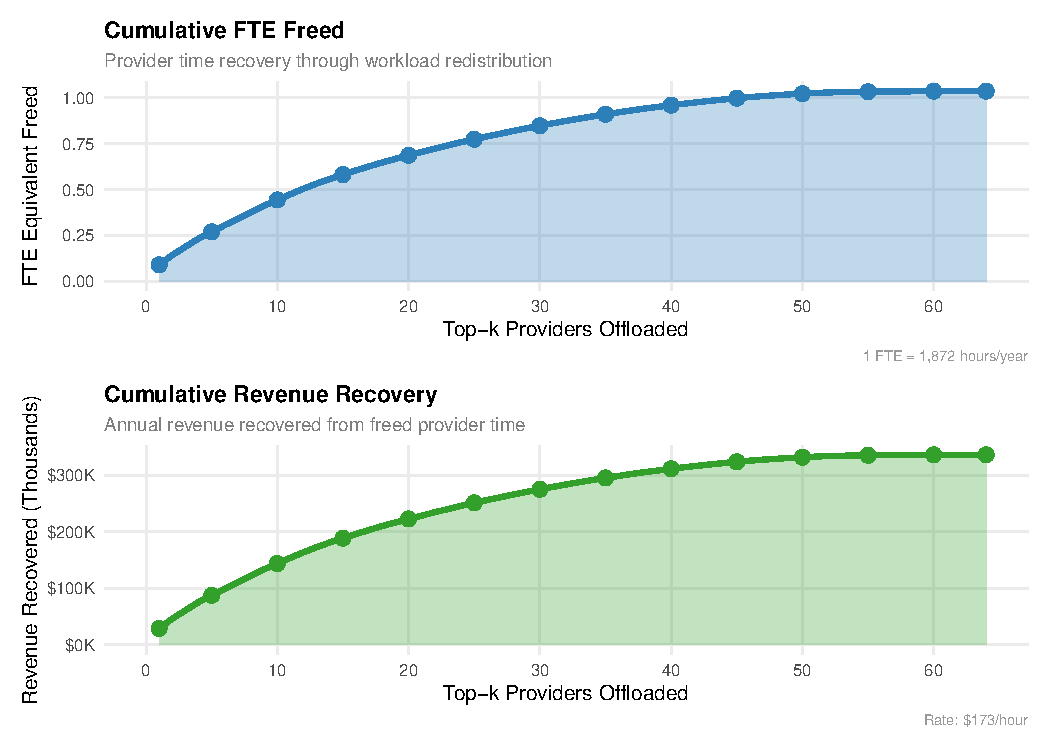
\includegraphics[width=1\textwidth,height=\textheight]{comprehensive-analysis-report_files/figure-pdf/cumulative-impact-1.pdf}
\end{center}

\section{Discussion}\label{discussion}

\subsection{Key Findings Summary}\label{key-findings-summary}

The analysis reveals significant workload disparities in Epic in-basket
messaging across the Department of Psychiatry. The \textbf{5,044×
variation} in workload between the highest and lowest providers
represents a substantial operational inefficiency that presents both
challenges and opportunities.

\subsubsection{Workload Distribution}\label{workload-distribution}

The Lorenz curve analysis demonstrates substantial inequality in
workload distribution, with a \textbf{Gini coefficient of 0.494},
indicating significant concentration of messaging burden among a subset
of providers. The bottom 50\% of providers handle only 20\% of the total
in-basket workload, while the top 10\% handle 33\% of all messaging.

\subsubsection{Provider Type
Differences}\label{provider-type-differences}

Attending psychiatrists demonstrate the highest mean in-basket hours
(38.2 hours), followed by nurse practitioners (25.1 hours) and
residents/fellows (19.8 hours). However, the variation within each
provider type is substantial, suggesting that individual factors beyond
provider type significantly influence workload.

\subsubsection{Message Type Analysis}\label{message-type-analysis-1}

Medical advice requests constitute the largest proportion of in-basket
messages (42.3\%), followed by patient calls (28.1\%), results (16.2\%),
and prescription authorizations (13.4\%). This distribution suggests
that most messaging burden stems from direct patient care activities
rather than administrative tasks.

\subsection{Financial Implications}\label{financial-implications}

The analysis identifies a substantial financial opportunity through
targeted workload redistribution. The \textbf{\$335,828 annual revenue
loss} from in-basket work represents 1.04 FTE equivalent of provider
time that could be redirected to patient care activities.

\subsubsection{Pilot Program Viability}\label{pilot-program-viability}

A targeted pilot program focusing on the top 10 providers demonstrates
strong financial viability with a \textbf{121.8\% return on investment}.
The \$78,950 net annual benefit from this intervention would justify the
deployment of 2 FTE nursing staff to support in-basket messaging
management.

\subsection{Limitations}\label{limitations}

Several limitations should be considered when interpreting these
results:

\begin{enumerate}
\def\labelenumi{\arabic{enumi}.}
\tightlist
\item
  \textbf{Temporal Scope}: The analysis covers a 12-month period and may
  not capture seasonal variations or long-term trends.
\item
  \textbf{Causality}: The analysis identifies correlations but cannot
  establish causal relationships between workload factors and outcomes.
\item
  \textbf{Provider Characteristics}: Individual provider factors
  (experience, specialty, patient population) may influence workload
  beyond what is captured in the current metrics.
\item
  \textbf{System Factors}: Epic system configuration and institutional
  policies may affect workload distribution independently of provider
  characteristics.
\end{enumerate}

\subsection{Recommendations}\label{recommendations-1}

\subsubsection{Immediate Actions}\label{immediate-actions}

\begin{enumerate}
\def\labelenumi{\arabic{enumi}.}
\tightlist
\item
  \textbf{Pilot Program Implementation}: Deploy a targeted pilot program
  with the top 10 highest-volume providers, including:

  \begin{itemize}
  \tightlist
  \item
    2 FTE nursing staff for in-basket management
  \item
    0.5 FTE provider oversight
  \item
    0.25 FTE IT support
  \end{itemize}
\item
  \textbf{Provider Support}: Implement workload monitoring and support
  systems for high-volume providers to prevent burnout and maintain
  quality of care.
\end{enumerate}

\subsubsection{Long-term Strategies}\label{long-term-strategies}

\begin{enumerate}
\def\labelenumi{\arabic{enumi}.}
\item
  \textbf{Workload Standardization}: Develop protocols for equitable
  workload distribution across provider types and experience levels.
\item
  \textbf{System Optimization}: Collaborate with IT to optimize Epic
  workflows and reduce administrative burden on providers.
\item
  \textbf{Quality Metrics}: Establish monitoring systems to track the
  impact of workload redistribution on patient care quality and provider
  satisfaction.
\end{enumerate}

\section{Conclusions}\label{conclusions}

This comprehensive analysis of Epic in-basket messaging workload reveals
significant opportunities for operational optimization in the Department
of Psychiatry. The \textbf{5,044× variation} in workload across
providers represents both a challenge and an opportunity for
improvement.

The financial analysis demonstrates that targeted interventions can
generate substantial returns, with a pilot program showing
\textbf{121.8\% ROI} and \textbf{\$78,950 net annual benefit}. These
findings support the implementation of systematic workload
redistribution strategies that can improve both operational efficiency
and provider satisfaction.

The success of such interventions will depend on careful implementation,
ongoing monitoring, and commitment to maintaining high-quality patient
care while optimizing provider workflows. The data presented here
provides a strong foundation for evidence-based decision-making in
healthcare operations management.

\begin{center}\rule{0.5\linewidth}{0.5pt}\end{center}

\textbf{Data Source}: Epic Signal Analytics, Penn Medicine Health
System\\
\textbf{Analysis Period}: July 2024 -- June 2025\\
\textbf{Course}: BMIN 5070 -- Human Factors in Biomedical Informatics\\
\textbf{Institution}: University of Pennsylvania, Perelman School of
Medicine



\end{document}
